%!TEX root = Intro-NLP-seminar.tex
\section{Aplicación a misiones espaciales}


\plain{However\ldots}




\begin{frame}[allowframebreaks]
\frametitle{Use cases of MT}
\framesubtitle{What do you need MT for?}
\textcite[ch.~10]{Somers:2003} pointed out 3 use cases of MT.
\begin{itemize}
\item \textbf{Disemmination}
	\begin{itemize}
	\item Translation output to be distributed for human as-is without changes
	
	
	
\framebreak
	\item Example Russian--English translation, suitable for dissemination:
		\begin{description}
		\item[Russian:] 18 февраля 2015 года Аналитическое управление аппарата Совета Федерации совместно с экономическим факультетом МГУ проводят научный семинар «Реалистическое моделирование».
		\item[English:] February 18, 2015 Analytical Department of the Federation Council in conjunction with the Faculty of Economics of Moscow State University conducted a scientific seminar ``The realistic simulation.''
		\end{description}
\framebreak
\item \textbf{Assimilation} 
	\begin{itemize}
	\item Just to get a rough idea of the content
	\item Output need not be perfect
	\item But choice of words should reflect original meaning

	 \end{itemize}
\framebreak
	\item Example Japanese--English translation, for assimilation:
		\begin{description}
		
		\item[English:] Attracts the brightest minds in the world, what What are the well-equipped environment support system, such as can concentrate on research.
		\end{description}
	\end{itemize}
\framebreak
\item \textbf{Interchange}
	\begin{itemize}
	\item Translation in one-to-one communication (telephone or written correspondence).
	\item Internet: tweets, blog posts, forums
	\item Human translation is out of the question (too slow)!
	\item \emph{Any} output (even if poor) is better than \emph{no} output
%	\item Usually for shorter phrases and values
%	\item Context is still important to choose correct words to reflect similar meaning!
	\end{itemize}
\end{itemize}
\end{frame}



\begin{frame}
\frametitle{Information Extraction (IE)} 

\begin{itemize}[<+->]
\item Extract ``interesting'' facts to store in a knowledge base 
\item `John stays in London. He works there for Polar Bear Design.'
	\begin{exampleblock}{Knowledge Base}
	$\text{John}_\text{PER} \xrightarrow{\text{live-in}} \text{London}_\text{LOC}$\\
	$\text{John}_\text{PER} \xrightarrow{\text{employee-of}} \text{Polar Bear Design}_\text{ORG}$
	\end{exampleblock}
\end{itemize}
\end{frame}


\begin{frame}
\frametitle{Another IE Example (Easier?)}
    
\begin{figure}
\centering
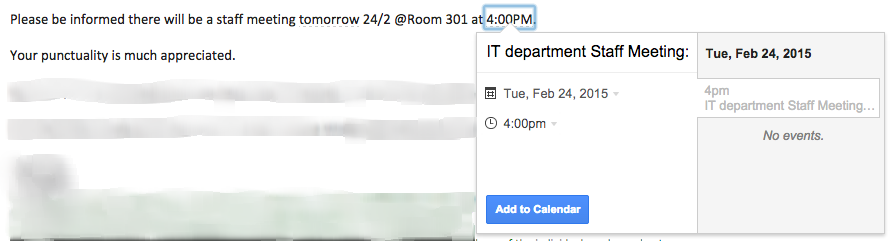
\includegraphics[width=\textwidth]{IE-event}
\end{figure}

NLP applications are often easier to design and implement with a specific use case scenario in mind

\end{frame}



